\chapter{Introduction and Motivation}
\label{ch:intro}


\section{Motivation}
\label{sec:motivation}


Since the discovery (and further confirmation) of the greenhouse effect in the years from 1824 to 1900 \cite{fourier1824remarques, foote1856circumstances} humans came a long way of fighting the consequences of the increased greenhouse gas concentration in earth's atmosphere. 
In 1972 \citeauthor{sawyer1972man} summarized the knowledge and predicted quite accurately the warming at the end of the century \cite{sawyer1972man}.
Especially the last decades the climate crisis gained more and more attention, leading to the creation of multiple international organizations and institutions (e.g. the International Panel on Climate Change (IPCC) in 1988).


\begin{figure}[hbt]
  \begin{center}
    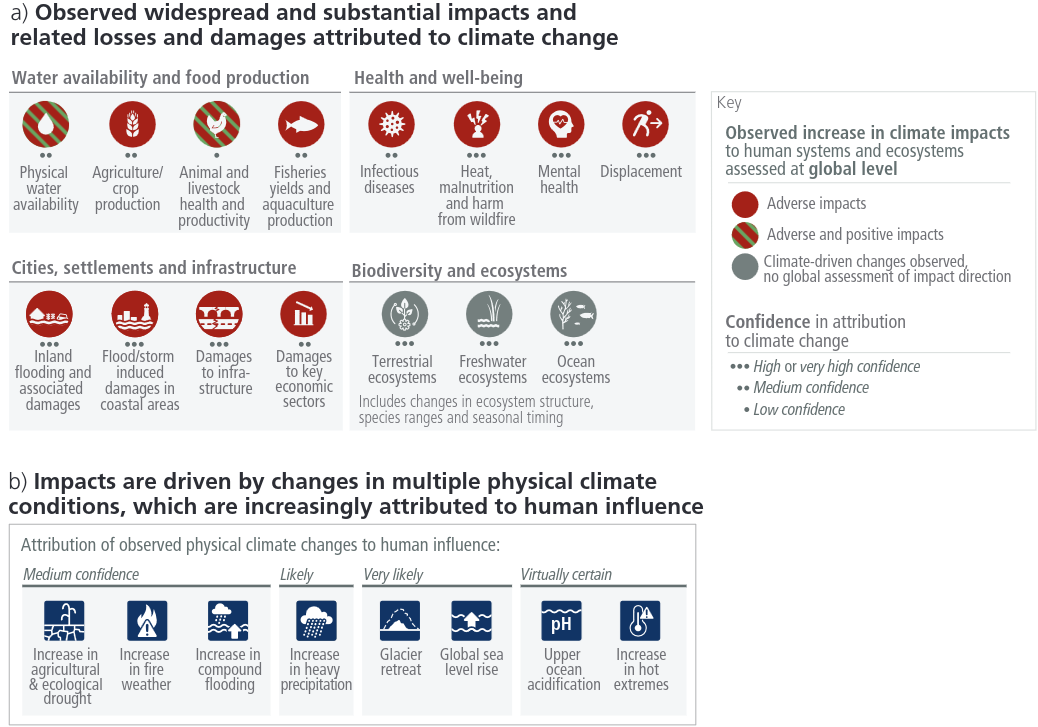
\includegraphics[width=0.65\textwidth]{figures/ipcc_6th_report_impacts_climate_change.png}
  \end{center}
  \caption{Impact of Climate Change for Humans, taken from \cite{lee2024climate}}
  \label{fig:impacts_climate_change}
\end{figure}



In 2019 more than 11,000  scientists from around the world released a declaration \cite{ripple_world_2019}, calling governments from around the world to action.
The consequences for the environment and humans are prevalent and are, in part, already visible today. 
Figure \ref{fig:impacts_climate_change} shows likely consequences for humans from the latest IPCC report for policymakers \cite{lee2024climate}: Flooding, malnutrition, displacement, and damages to all kinds of ecosystems can be attributed with high confidence to climate change. 
The sources of such consequences are manyfold, but recent research shows that big circulation systems like the North Atlantic Oscillation\cite{vietinghoff_visual_2021} or the Atlantic Meridional Overturning Circulation \cite{lobelle_detectability_2020} change as well. 
% The mid and long-term consequences are manyfold and go far beyond the general rising of the worlds' average temperature (see Figure \ref{fig:impacts_climate_change}), e.g. shifts in circulation systems like the North Atlantic Oscillation (NAO) \cite{vietinghoff_visual_2021}, which in turn also have varying consequences. 

Although the water vapor in the air accounts for only 0.001 \% of the water on the earth, it is the most active part of that cycle \cite{zou_investigating_2020}. 
Also, research shows that the precipitation on land does not match the evaporation, meaning the water was transported (from the oceans) to land, providing water for the ecosystems there.  \todo{CITE!!! Where the fuck did I read this?}
Analyzing the structural change of this moisture transport could help predict consequences. 
Motivated by the research of \citeauthor{vietinghoff_visual_2021}, this thesis aims to evaluate similarly the systemic changes of moisture transport patterns in Europe and the northern Atlantic. 


\section{Climate and Climate Research}
\label{sec:climate}

% This section should give an introduction to the current state of climate research. 
% Therefor it should explain what the current way of future climate predictions is (Coupled Models), how they work, and 
% It should explain some part of the politics, who is involed in what and what the backroud of the most important projects (CMIP, ScenarioMIP \dots). 
% It should be explained that the data used is the one that the highest council of fighting climate change uses for its report. 


\subsection{Quick Overview over Climate Systems and Climate Change}

% Contents of this section: 
%
% \begin{itemize}
%   % \item What are climate systems? 
%   % \item What are forcings? 
%   \item What does variability in climate systems stem from?
%   \item Give an example with the NAO
% \end{itemize}

In difference to weather, which is the momentary state of the atmosphere at a time, climate is the average of weather patterns over a larger period of time, usually 30 years or more \cite{noaa_whats_nodate}. 
So the term climate change does not refer to any unexpected weather changes, but to the structural changes of said patterns over a large period of time (e.g. the warming of the global average temperature). 
Earth's climate system can be seen as complex interactions of its major components: atmosphere, hydrosphere, cryosphere, lithosphere, and biosphere \cite{vietinghoffdiss, intergovernmental_panel_on_climate_change_ipcc_climate_2023}. 
Changes in this system can have (roughly) two reasons: 
Either \enquote{internal variations in form of redistributions of energy} \cite{vietinghoffdiss}, which can happen on arbitrary scales (see the discussion on the change of AMOC in \cite{lobelle_detectability_2020}) or in the form of external forcings. 
Such forcings could be vulcanic activity, differences in solar radiation, and of course the emission of greenhouse gases (GHGs). 

\begin{figure}[htb]
  \begin{center}
    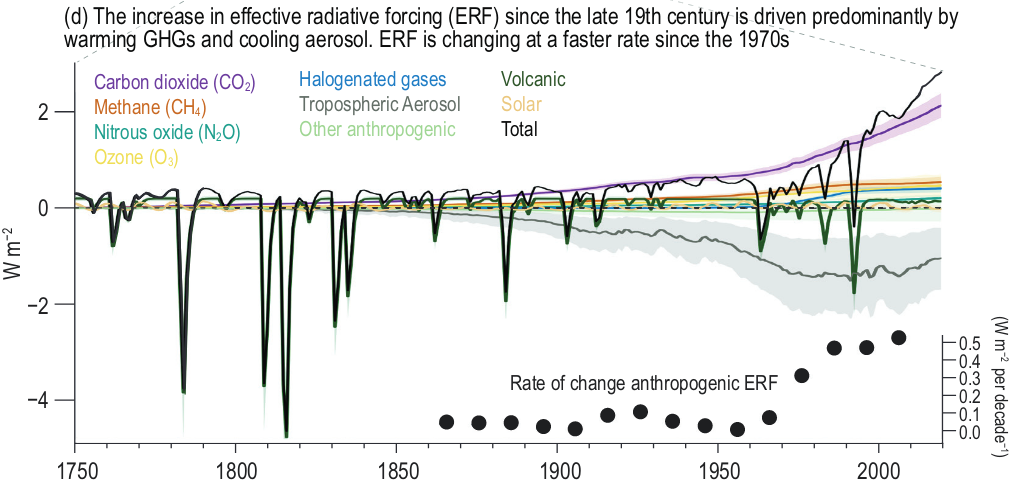
\includegraphics[width=0.95\textwidth]{figures/ERF_change_with_forcings.png}
  \end{center}
  \caption{The evolution of the effective radiative forcing and contributing components, taken from \cite{intergovernmental_panel_on_climate_change_ipcc_climate_2023}}\label{fig:erf-with-forcings}
\end{figure}

Figure \ref{fig:erf-with-forcings} gives an example what effect such external forcing can have: It shows the change in effective radiative forcing (ERF) and its contributing components. 
ERF (in $Wm^{-2}$) is a way of measuring how much energy from the sun is \enquote{trapped} instead of reflected back to space (greenhouse effect). 
A positive value means warming, while a negative value is associated with cooling. 
In can be seen in Figure \ref{fig:erf-with-forcings} that neither volcanic activity or solar radiotian changed that much, the main drivers of change in ERF are the man-made GHGs and cooling aerosols. \cite{intergovernmental_panel_on_climate_change_ipcc_climate_2023}

Regarding the internal variations: Most of it is part of some oscillation, with the oscillations of the atmosphere with the hydrosphere (i.e. all liquid forms of water on earth) being responsible for large parts of climate's internal variations on decadal and interannual time frames \cite{vietinghoffdiss}. 
Prominent examples for such oscillations are the El Niño Southern Oscillation (ENSO) or the North Atlantic Oscillation (NAO), which is especially relevant for this thesis. 


\subsection{The North Atlantic Oscillation}

The aforementioned NAO is \enquote{... one of the most recurrent and prominent patterns of atmospheric circulation variability} \cite{hurrell_overview_2003}. 
It is also one of the oldest known weather patterns, since some descriptions of Scandinavians exist from a few centuries back. 
It dictates the climate variability for a large area: From the East Coast of the USA to Siberia and from the Arctic to the subtropical Atlantic.
Especially in the boreal winter (usually from December to February), the variations of the NAO influences a wide range of variability areas: From the mean wind speed and direction to the heat and moisture transport as well as the intensity and amount of storms and their path. 

\begin{figure}[htb]
  \begin{center}
    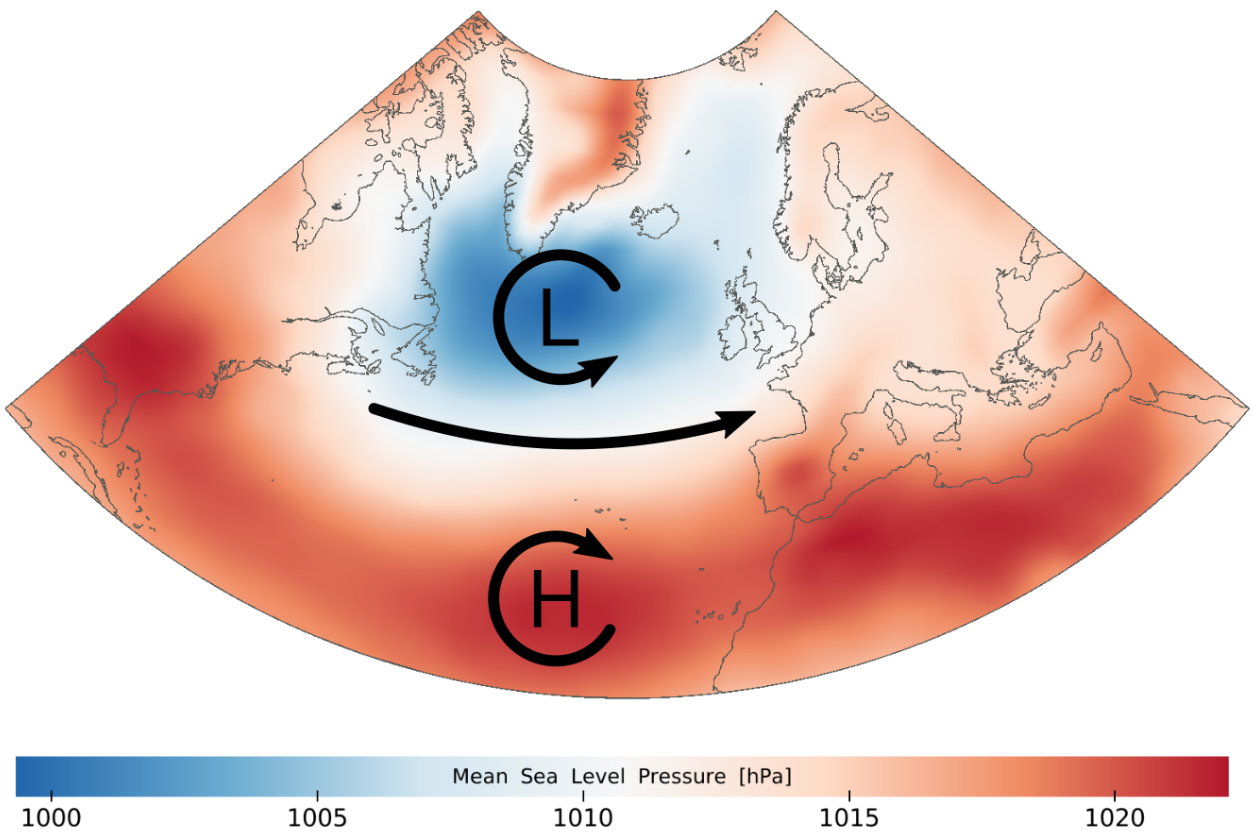
\includegraphics[width=0.95\textwidth]{figures/nao_pattern_diss.png}
  \end{center}
  \caption{Characteristic mean SLP field of a boreal winter season, taken from \cite{vietinghoffdiss}. It shows a high (H)/low (L) pressure pattern, directing air from the Atlantic westwards towards Europe. }
  \label{fig:naopattern}
\end{figure}


The NAO is a redistribution of atmospheric mass from the Arctic to the subtropical Atlantic, producing the aforementioned effects while swinging from one phase to another. 
It's basis is a characteristic dipole in the Sea Level Pressure Field (SLP) of the Atlantic (see Figure \ref{fig:naopattern}).
Due to the Coriolis Force, air flows clockwise around high pressure and counterclockwise around low pressure in the Northern Hemisphere, leading to the transport of the maritime air from the Atlantic towards Europe (see Figure~\ref{fig:naopattern}) \cite{hurrell_overview_2003, vietinghoffdiss}. 
Depending on the pressure differences, the effect varies: High pressure differences lead to higher transport of mild, humid air to Europe, which in turn results in milder European winters. In contrast, a low difference leads to a less pronounced effect and therefor to colder winters. 
This varies on an interannual scale, and this effect is called the North Atlantic Oscillation. 
The difference per year is called the NAO index and can be seen in Figure \ref{fig:naoindex_comparison}. 


\begin{figure}[htb]
  \begin{center}
    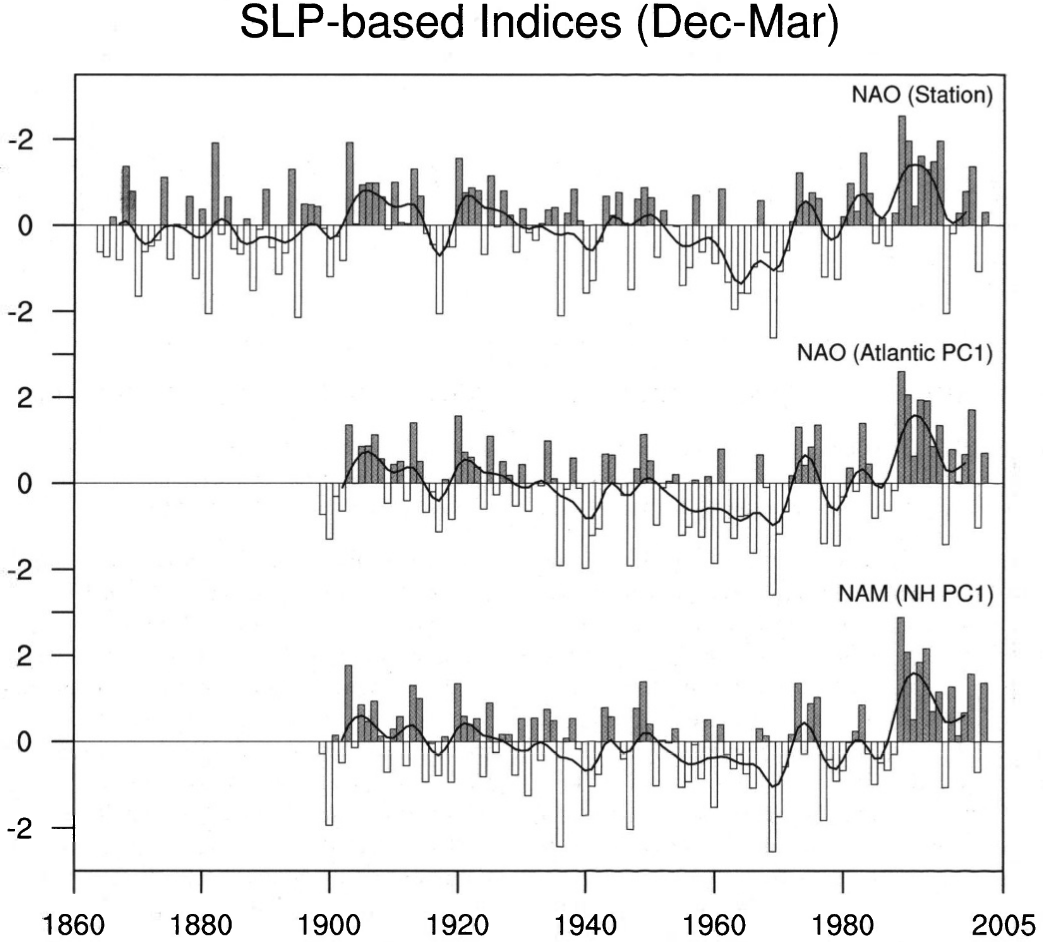
\includegraphics[width=0.75\textwidth]{figures/hurrel_nao_index_comparison.png}
  \end{center}
  \caption{Comparison of the NAO index from \cite{hurrell_overview_2003}: The top panel are differences of SLP from weather stations in Portugal and Iceland, the middle panel is the first principal component of corresponding to the first EOF of the northern Atlantic SLP field, and the bottom panel is the same as the middle panel but for the whole Northern Hemisphere. See \cite{hurrell_overview_2003} for a more detailed description}
  \label{fig:naoindex_comparison}
\end{figure}

A large fraction of the recent warming in Europe can be linked to the behavior of the NAO in the last decades: it shifted from large amplitude anomalies in the negative to similar anomalies in the opposite direction in the later years. 
Therefor, \citeauthor{hurrell_overview_2003} points out the need to study the relationship of anthropogenic climate change and the NAO. 
Following this, the motivation of thesis \cite{vietinghoff_visual_2021} by \citeauthor{vietinghoff_visual_2021} tried to track the shift of the centers of the dipoles in different climate scenarios.   


\subsection{Climate Research: The IPCC and the Coupled Model Intercomparison Project (CMIP)}


The reason for the endorsement of the IPCC by the UN General Assembly 1988 was to prepare comprehensive reviews and report about the current state of scientific knowledge and research. 
Since then there were six assessment cycles and six reports were published, condensing the research of the scientific community. Figure \ref{fig:impacts_climate_change} is a graphic from the latest report for policymakers from 2023 \cite{lee2024climate}, displaying the probable consequences for humans in climate change.

A main source for such figures in the reports are so-called Global Coupled Models (GCMs)\footnote{Unfortunately, Global Coupled Models share their acronym with General Circulation Models, which are quite similar}, trying to model the state and evolution of certain fields of earth data.
They consist of multiple Models, each representing a major part of Earth's complex climate system (like atmosphere, hydrosphere, etc.), also allowing to model the dynamic interactions between these parts \cite{vietinghoffdiss}. 
In the mid 90s the Coupled Model Intercomparison Project (CMIP) was brought to life, with the aim of streamlining results of GCMs and making them comparable. 
CMIP provides the outer structure, amongst others what kind of simulations to produce (e.g. preindustrial control simulations, future scenarios etc.), what kinds of fields should be generated, what kind of resolutions to provide and also how these results should be serialized.
Since then the results of CMIP played an increasingly major part in the reports of the IPCC \cite{touzepeiffer_coupled_2020}, and are now even called \enquote{... one of the foundational elements of climate science} \cite{eyring_overview_2016}. 
CMIP is currently in its 6th phase, corresponding to the recently finished 6th Assessment Report of the IPCC \cite{lee2024climate}. 
The 6th phase describes an inner core (DECK + historical simulations), required for participating in CMIP, and some endorsed Model intercomparison Projects (MIPs). 
The latter are optional and consist of e.g. ScenarioMIP (future scenario simulations), HighResMIP (for exploring Models with higher resolutions), and GeoMIP (exploring effects of geoengineering).


\section{Research Questions and Thesis Structure}
\label{sec:research_questions}

Following up the previous sections, the research question for this thesis is: 

\begin{center}
  \larger{\enquote{How do the Patterns of Moisture Transport change in the face of various climate scenarios in the North-East Atlantic?}}
\end{center}


The remaining thesis is structured as follows: Chapter \ref{ch:basics} gives the theoretical background on fields and pattern analysis. 
The following Chapter \ref{ch:dataset} gives a detailed overview about the used CMIP6 based dataset. 
Chapter \ref{ch:related_work} provides an overview of related work, the motivation for this thesis and the placement of this thesis in the academic context. 
While the results are discussed and presented in Chapter \ref{ch:results}, Chapter \ref{ch:methodology} gives a detailed description how these results came about. 
The thesis is concluded with Chapter \ref{ch:conclusions} and gives an outlook for future research. 

